\documentclass{sig-alternate}

\begin{document}
%
% --- Author Metadata here ---
\conferenceinfo{CIKM}{'2016 Indianapolis, IN USA}

\title{What makes a query temporally sensitive?}

\maketitle
\begin{abstract}
Here is the abstract
\end{abstract}

% A category with the (minimum) three required fields
\category{H.4}{Information Systems Applications}{Miscellaneous}

\terms{}

\keywords{}

\section{Introduction}

A basic intuition in temporal information retrieval research is that time should be modeled explicitly when scoring and ranking documents with respect to users' queries. Users' criteria of recency, currency, and freshness have long been recognized as factors when judging relevance \cite{Barry1998}.  A number of studies have investigated the role of time in information retrieval using a variety of methods including query log analysis \cite{Kulkarni2011,Shokouhi2011,Metzler2009}, temporal expression extraction \cite{Berberich2010, Kanhabua2011}, temporal distribution of pseudo-relevant documents \cite{Jones2007}, and temporal retrieval models \cite{Li2003, Efron2011, Dakka2012}.  These researchers refer to general classes of ``temporal queries'' and ``temporal information needs.''  Models have been proposed and evaluated for ``recency queries'' \cite{Li2003, Efron2011}, ``time-sensitive queries'' \cite{Dakka2012}, ``implicitly temporal queries'' \cite{Metzler2009}, and ``temporally biased queries'' \cite{Jones2007}.  In a widely cited study, Jones and Diaz propose three different ``temporal classes of queries'' \cite{Jones2007}.  

In this paper, we explore the question what \emph{what makes a query temporally sensitive?} 

To address this question, we analyze over 600 topics previously used in the experimental evaluation of temporal retrieval models. In four previously published studies \cite{Jones2007, Efron2011, Dakka2012, Peetz2013}, researchers manually classified standard TREC topics as either ``temporal'' or ``non-temporal.'' In this study, we employ qualitative techniques to identify and annotate characteristics of topics that might affect manual assessment of ``temporality.'' The resulting coded topics are used in a regression analysis to determine the specific relationships between these characteristics and manual assessment of topic temporality. Finally, we use the coded topics to predict which topics might benefit from temporally-sensitive retrieval models.

This paper is structured as follows.  In section 2, we review the concept of information needs. In section 3, we review the role of time in information retrieval research. 


To address this question, we first review how researchers have approached investigations of the role of time in information retrieval. We survey the literature, focusing on methods of analysis, definitions, and operationalizations of time-related concepts. We then report the results of our analysis of over 600 topics previously used in experimental evaluation. 


\section{On information needs}

The concept of \emph{information needs} has been extensively discussed in the information science literature and is widely used in the information retrieval community. While many theories have been proposed, no single definition is widely accepted.  Synthesizing theories proposed by Taylor \cite{Taylor}, Wilson \cite{Wilson}, and Cole \cite{Cole}, here we define an \emph{information need} as the unobservable motivation behind individual users' information seeking. Information needs reflect the individual user's current state of mind and context, including social and cultural environments. While information needs themselves are not observable, user's information seeking behaviors -- including queries and document relevance judgements -- are incomplete but observable evidence of the underlying need. Due to the individual nature of information needs, no two are identical, but given social and cultural contexts many needs are expressed by similar queries and satisfied by similar documents. 

We believe that this definition captures the spirit of the concept of \emph{information need} as commonly used in information retrieval research, particularly in the case of ``topics'' in the Text REtrieval Conference (TREC).

\section{A brief history of time in IR}

Early evidence of temporal information needs can be found in descriptive and subject cataloging practice employed in library catalogs. Library cataloging predates online information and in many ways reflects the historical needs of users. Descriptive and subject cataloging practice capture a variety of temporal characteristics of published resources including publication dates, copyright dates as well as chronological terms intended to facilitate subject searching based on particular periods of time. While publication dates capture when a resource was published or created, chronological terms and subdivisions (e.g., Wars of the Roses, 1455-1485) in subject headings indicate if a resource is \emph{about} a particular period in time. 

With regard to time, descriptive cataloging is primarily concerned with production dates. This includes publication dates, distribution dates, and copyright dates. In the event that publication dates are not present, catalogers often provide approximate dates based on their knowledge and experience.  Publication date information allows users to search for resources based on temporal constraints (e.g., date range) or to rank results based on the most recent or oldest publication dates. 

Subject cataloging, on the other hand, is concerned with the topical content of the work.  Subject headings lists, such as the Library of Congress Subject Headings (LCSH), include a variety of different methods for specifying temporal content \cite{Chan1972}.  Subject headings allow users to search for resources based on temporal (or chronological) content. 

These cataloging practices suggest two distinct classes of temporal information needs: those based on the ability to find resources published at particular points in time and those based on the ability to find resources about particular periods in time. Of course, an information need may combine the two (e.g., find books about the Wars of the Roses published in the 1800s). We will refer to these as \emph{temporal relevance} and \emph{temporal topicality}.
 
\subsection{Time and relevance}

In two separate studies of user criteria for judging document relevance, Barry and Schamber \cite{Barry1998} both found \emph{recency} (or \emph{currency}) to be an important characteristic for some users and information needs.  They define this as ``the extent to which users judged information to be current, recent, up-to-date, or timely.'' \cite{Barry1998}  In Barry's analysis of 18 interview respondents, ``currency'' was the sixth most-mentioned out of 21 different relevance criteria.  In Schamber's study of 30 respondents, it was the second most-mentioned to of 10 different relevance criteria. 

The concept of \emph{recency} is related to the later concept of \emph{freshness} found in research focused on web search \cite{Dai}. In web search, \emph{freshness} is related to the time when a web page or link was last updated. \cite{Berberich2005}  Research has consistently found that users prefer (and thus judge as more relevant) resources that are more frequently and recently updated.  Prior to the web, \emph{recency} was primarily represented by document publication dates. 

Another role of time in the judgment of relevance is suggested by Mizzaro \cite{Mizzaro1997}, who observes that, as the user learns things or the problem changes, a document may not be relevant to a query at one point in time, but be relevant later (or vice versa).  This type of user-dependent temporal relevance can be described as \emph{temporal relevance dynamics} -- how the relevance of a document with respect to an information need may change over time. While Mizarro is concerned mainly with changes in the users' state of mind, as we will discuss later, what is considered relevant can also change at an aggregate level for many users.

So far, we have identified three broad classes of temporal information needs: 1) instances where document publication dates matter; 2) instances where the topics are periods in time; and 3) instances where what is relevant changes over time. Following Jones and Diaz, we can add to this the negative case 4) when time is not a factor at all.

\subsection{Temporal query dynamics}

Informally, the study of \emph{dynamics} is concerned with characteristics that stimulate changes in a system or process. We use \emph{temporal dynamics} to refer to the specific study of change with respect to time. Whereas \emph{temporal relevance dynamics} focuses on the study of how what is relevant to users changes over time, \emph{temporal query dynamics} focuses on the study of queries over time. \cite{Kulkarni2011}

Studies of temporal query dynamics generally focus on the analysis of query streams in the form of search engine logs. These studies have identified classes of temporal patterns in query streams (e.g., seasonal/periodic \cite{Shokouhi2011}, bursts \cite{Vlachos2004}, trends \cite{Parikh2008}) as well as methods for identifying these patterns and using them for the classification of queries or correlation with external events \cite{Lavrenko2000,Vlachos2004}.

One of the more compelling studies in this area is that of Kulkarni et al \cite{Kulkarni2011}.  The authors combine multiple sources of information -- query logs, click-through logs, web crawler content changes, and human relevance judgments -- to understand the relationship between query dynamics, relevance dynamics, and content dynamics. They study how time impacts which queries are issued, which documents are deemed relevant, and how changes in the content of documents relate to relevance judgments.

Queries are observable evidence of users' information needs. Patterns of similar queries and similar judged-relevant documents over time suggest that certain queries reflect common  underlying information needs. These studies indicate that some queries are repeated over time, others occur at particular points in time, and that query intents also change over time.   That is, the same query surface form may represent distinct information needs and be satisfied with different documents at different points in time.

Returning to our motivating question, these studies suggest additional conditions. The ``intent'' of commonly-issued queries, and therefore which documents satisfy these queries, can change over time. Changes in query intent can be one-time, as the primary or dominant intent changes due to shifts in popularity, or periodic: at different times of day, days of the week, or days in the year. In each of these cases, documents that are likely to be relevant to a particular query depend on when the query is issued.


\subsection{Temporal topicality}

Metzler et al \cite{Metzler2009} investigate \emph{implicitly year qualified queries} which they indicate are a subset of ``temporal queries.'' They define a ``year-qualified query'' as a query containing a year and an ``implicitly year-qualified query'' as a query where the user might have a specific year in mind.  Examples include ``miss universe,'' ``olympics,'' ``easter,'' and the names of annual conferences.  The study is based on the analysis of query logs, with time operationalized by the presence or absence of years in the query string. 

Year qualified queries are in one sense temporally-topical queries.  Users are primarily concerned with content about the year qualified topic, not with information published at a particular point in time. In the examples provided, year qualified queries are also periodic or seasonal, referring to events that occur on an annual basis. It is reasonable to suggest that implicit year qualified queries are a type of recency query, where users are interested in the most recent or up-to-date information about a periodic event. This suggests that queries concerning periodic events may combine temporal-topicality and temporal relevance.

Taking a different approach, Berberich et al \cite{Berberich2010} propose an extension to the language modeling framework for information retrieval that incorporates information derived from temporal expressions.  Example queries include ``fifa world cup 1990s'' or ``13th century crusades.'' Their basic approach is to extract temporal expressions from queries and documents and convert them to the time domain. Documents are then scored based on their query likelihood with regard to the textual content combined with the likelihood given the temporal coverage of the document in the time domain.

The authors develop a test collection based on the New York Times Annotated Corpus.  Two different human intelligence tasks (HITS) were developed using the Amazon Mechanical Turk (AMT) service. In the first task, users were given entities related to a subset of topics (sports, culture, technology, and world affairs) and asked to specify a temporal expression for the entity. In the second task, users were shown a temporal expression and asked to select and entity from the topics. From these tasks, 40 queries were selected. Examples include ``boston red sox [october 27, 2004],'' ``pearl harbor [december, 1941],'' ``sewing machine [1850s],'' and ``muhammed [7th century].''   Relevance assessments were collected using AMT.

The test collection developed by Berberich et al is important, as it is used for this and several subsequent studies. The authors rejected the idea of using existing test collections because they need ``a specific class of information needs'' represented by queries with explicit temporal expressions.  There are several interesting characteristics of this test collection.  First, the document collection is a corpus of news articles. As we will see in the next section, news articles are a common document type for temporal retrieval research.  Second, the queries are developed around ``entities'': people, organizations, places, and products. A review of the 40 queries indicates that over 50\% contain either names of people or organizations. This suggests one of three things: 1) queries in general are primarily about named entities; 2) explicit temporal expressions occur primarily with respect to named entities; or 3) it's easier to construct queries with temporal expressions with respect to named entities.  

Kanhabua and Norvag \cite{Kanhabua2011} explore ``time-aware retrieval models'' using Berberich's NYT corpus. They use a similar justification, that TREC ``queries are not time-related, and judgments are not targeted towards temporal information needs.'' In addition to temporal expressions found in the document content, they also incorporate temporal information based on the document publication time. Both content time and publication time are used with respect to the explicit temporal expression found in the query.

\subsection{Time-sensitive queries}
Li and Croft's study of ``recency queries'' was the first in a line of research focused on what we have termed \emph{temporal relevance}. Temporal relevance is concerned with conditions where documents published at particular points in time are considered more or less relevant than those published at other times. This condition is studied independent of or in conjunction with traditional topical retrieval models.  In this section, we review how researchers operationalize the concept of time and define the temporal characteristics of queries in their studies. 

Li and Croft \cite{Li2003} hypothesize that some queries are ``recency queries'' where the most recently published documents are more likely to be relevant. They analyze queries associated with TREC topics 301-400 from TREC disks 4 and 5. Through the direct analysis of the temporal distribution of judged relevant documents, they classify 36 of the queries as recency queries because they have ``more relevant documents in the recent past.''

There are two problems with this approach. First, the distribution of judged relevant documents is not conclusive evidence that the query is temporally constrained. There are a variety of reasons why judged relevant documents may appear primarily in the recent past. Second, the authors did not recognized a potential problem in the underlying document collection.  For their analysis, they used TREC 8 (disks 4 and 5), which consists of timestamped newswire documents from the Financial Times (1992-1994), Los Angeles Times (1989-1990), and the Foreign Broadcast Information Service (1994).  Each of these sub-collections has distinct temporal characteristics that, when combined, may be misleading. Figure X shows the temporal distribution of results for query 301, a motivating example from their paper.  Looking at the overall distribution of results from TREC 8, this appears to be a compelling example of a recency query.   However, looking at the distribution of results for each sub-collection, we can clearly see that the ``recent'' results are those that appear in the FBIS collection.  Further analysis indicates that the ``recency'' queries identified by Li \& Croft are dominated by queries with results in FBIS.  This suggests that temporal retrieval models should be evaluated against individual sub-collections and that the temporal profile of collections is an important factor.  Because of this, the results of Li \& Croft's study as well as the identified ``recency'' queries should not be used further.

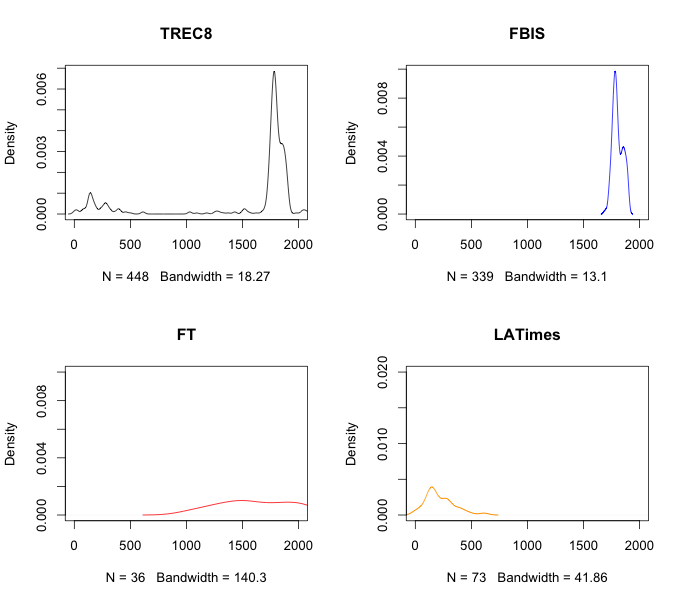
\includegraphics[width=8cm]{images/301.png}

Jones and Diaz \cite{Jones2007} study the temporal characteristics of queries with the goal of query classification through the analysis of three TREC news collections and a web search engine log. They use the Associated Press (1988, 1989) and Wall Street Journal (1990-1992) collections from TREC disks 1 and 2 as well as the AQUAINT corpus with the 2003 Novelty track topics. They defined three classes of queries based on the temporal distribution of pseudo-relevant documents: temporally ambiguous (requesting multiple events),  temporally unambiguous (requesting a single event), and atemporal (had no preference). They employed annotators to  manually classify 100 TREC queries based only on the topic title, description, and narrative.  Interestingly, they found that the queries were only atemporal or temporally ambiguous.  The 2003 Novelty track includes topics classified as ``event'' or ``opinion,'' which the authors found to correspond to the ``temporally unambiguous'' and ``atemporal categories.''  

We note a few things from this study, which will be discussed further later. First, the analysis is focused on news collections and search engine logs. Second, topics and relevance judgments were taken from existing TREC test collections.  Third, the notion of ``temporality'' is somehow related to ``events.'' 

Expanding on the work of Li and Croft, Dakka et al \cite{Dakka2012} investigate a broader class of queries which they refer to as ``time-sensitive.'' They hypothesize that there are queries where more relevant documents are found at specific points in time, not just recent.  They evaluate their models using two different test collections: a subset of TREC disks 4 and 5 and a custom test collection based on the Newsblaster news service.  Similar to Li and Croft, for the TREC collection they manually identify a subset of queries from topics 301-450 that they consider to be ``time-sensitive.'' To do so, they manually examine the title, description and narrative of each topic and identify queries associated with specific news events. If the topic information is insufficient to make a decision, they analyze the distribution of relevant documents.  Only those queries with more than 20 matching documents \footnote{based on conjunctive Boolean queries} were considered.  This resulted in a collection of 86 temporally sensitive queries. The document collection used for evaluation was restricted to the Financial Times (1991-1994) and Los Angeles Times (1989-1990) sub-collections, since they include timestamps. The second test collection was developed based on a six-year archive of Newsblaster, covering news articles from September 2001 to December 2006. The authors recruited five journalists who volunteered queries.  From 125 collected queries, 76 were identified as time-sensitive. Relevance judgments were collected using AMT.

Here we have another example of an analysis based on news collections where the central concept of a ``time-sensitive'' query is related to ``specific news events.'' Queries were identified through manual analysis of the topic text and the ground truth relevance judgments.

Further expanding on the work of Li and Croft, Efron and Golovchinsky \cite{Efron2011} investigate additional models for recency queries.  They use subsets of several TREC ad-hoc collections including the Associated Press documents from disks 1 and 2 with topics 101-200; Los Angeles Times and Financial Times documents from disks 4 and 5 with topics 301-450.  They classify queries as ``recency'' or ``non-recency'' based on an analysis of the distribution of relevant documents. If at least 2/3 of relevant documents appear after the median document time, the query is considered a candidate for recency.  Candidate queries are then manually reviewed to determine if they have a ``bona fide'' temporal dimension. However, the criteria for manual review were not specified.   The authors developed a second test collection using the Twitter API.  Two users of an experimental Twitter search engine were asked to create two types of queries: recency and non-temporal. Recency queries were defined as ``queries where relevant tweets were necessarily written recently.''  Relevance judgments were collected via AMT.  

In this case, we see a combination of news and social media where queries are classified based on manual review and analysis of judged-relevant document distributions.

In a more recent study, Peetz, Meij, and Rijke \cite{Peetz2013} investigate the effect of temporal bursts in estimating query models. Building on the above studies, they evaluate their models using several previously used collections (AP, LA Times, Financial Times). In addition, they introduce the Blogs06 collection.  As previously, the authors construct a subset of ``temporal'' queries through manual evaluation of topic descriptions and relevant document distributions. 

What can we conclude from these studies? First, each operationalizes time using the publication timestamp, which requires the availability of reliably timestamped document collections for evaluation.  Most of these studies rely on collections of news articles, but more recent research also incorporates social sources. Of the 10 studies reviewed, 8 use newswire collections, 3 use Twitter, 2 use blog collections, and 1 uses a standard web collection\footnote{This is by no means an exhaustive list of work in this research area}.  Second, there is no standard approach for identifying ``time-sensitive'' queries. Some studies rely on the analysis of the temporal distributions of judged-relevant or pseudo-relevant documents, others on the manual analysis of topic descriptions, and some on a combination of the two.  It is not clear from these studies how one determines whether a query is truly temporal or not.  Third, temporally-sensitive queries are apparently related to ``events.'' Jones and Diaz refer to the presence/absence of events in the manual analysis of topics. They also rely on the ``event'' category in the 2003 Novelty track.  Dakka et al consider queries temporally sensitive if they are ``associated with specific news events.''  Peetz, Meij, and Rijke assert that the proposed model ``detects events.''  Unfortunately, none of these studies provides any definition or direction as to how to operationalize the concept of an ``event.''

\subsection{Topic detection and tracking}

Much the research discussed so far is concerned primarily with using temporal characteristics in ad-hoc retrieval. A related area of research also concerned with time is that of document filtering. Whereas ad-hoc retrieval focuses on ranked lists of documents searched retrospectively, filtering is focused on decisions about document relevance made at specific points in time. Given a time-ordered stream of documents, systems must determine whether to emit or not emit a document when it is received, under certain constraints.  Sub-areas of filtering research are often focused on specific tasks such as topic or event detection. 

The Topic Detection and Tracking (TDT) program was developed by NIST and ran for seven years.  Two central tasks in the TDT program are 1) \emph{topic detection} to detect emerging topics in news streams and 2) \emph{topic tracking} to track those topics as they develop. TDT is the precursor to the recent Knowledge Base Acceleration (KBA) and Temporal Summarization tracks in TREC. In all of these cases, the goal is to monitor a stream of documents for changes that occur to specific information needs or topics.

The 2004 TDT Annotation Manual provides the following definitions for topics and events:

\begin{enumerate}
\item \emph{event}:  a particular thing that happens at a specific time and place, along with all necessary preconditions and unavoidable consequences. A
TDT event might be a particular plane crash, or a single meeting, or a particular court hearing. 
\item \emph{activity}:  a connected set of events that have a common focus or purpose, happening at a specific place and time; for instance, a
campaign, or an investigation, or a disaster relief effort. 
\item \emph{topic}: an event or activity, along with all directly related events and activities. 
\end{enumerate}

In TDT, events must be one of thirteen \emph{seminal events} and specific guidelines are provided as to what types of events are considered related.  In this sense, the \emph{topic} is the seminal event. The seminal event types and  examples from the 2004 Annotation Manual are listed in Table \ref{table.tdt}. 

\begin{table*}
\center
\small
\begin{tabular}{| p{3cm} | p{12cm} | }
\hline
\bf{Seminal event} & \bf{Examples} \\ \hline
elections & a specific political campaign, election day coverage, inauguration, voter turnouts, election results, protests, reaction  \\ \hline
scandals/hearings & media coverage of a particular scandal or hearing, evidence gathering, investigations, legal proceedings, hearings, public opinion coverage \\ \hline
legal/criminal cases &  the crime itself, arrests, investigations, legal proceedings, verdicts and sentencing  \\ \hline
natural disasters &  weather events (El Nino, tornadoes, hurricanes, floods, droughts), other natural events like volcanic eruptions, wildfires, famines and the like,
rescue efforts, coverage of economic or human impact of the disaster \\ \hline
accidents & transportation disasters, building fires, explosions and the like \\ \hline
acts of violence or war & a specific act of violence or terrorism or series of directly related incidents (such as a strike and retaliation) \\ \hline
science and discovery news & announcement of a discovery or breakthrough, technological advances, awards or recognition of a scientific achievement \\ \hline
financial news &  specific economic or financial announcements (like a specific merger or bankruptcy announcement); reactions to the event; direct impact on the economy or business world) \\ \hline
new laws & announcement of new legislation or proposals, acceptance or denial of the legislation, reactions. \\ \hline
sports news &  a particular sporting event or tournament, sports awards, coverage of a particular athlete's injury, retirement or the like.  \\ \hline
political and diplomatic meetings &  preparations for the meeting, the meeting itself, decisions, outcomes, reactions \\ \hline
celebrity and human interest news &  most often involves the death of a famous person or other significant life events like marriage \\ \hline
miscellaneous news & specific events or activities that do not fall into one of the above categories \\ \hline
\end{tabular}
\center
\caption{TDT seminal events and examples}
\label{table.tdt}
\end{table*}

The TDT research program is concerned with real-time filtering of time-ordered streams of documents, In this case, there is no topic or information need. Instead, systems are challenged to identify and track topics over time. Topics are related to the concept of an \emph{event} or \emph{seminal event}.  The collection is composed of timestamped new articles.


\section{What makes a query temporally sensitive?}

Queries represent a user's underlying information need and are issued over a collection at a particular point in time.  A single information need is often represented by multiple related queries issued over time. In this sense, a set of queries can be seen as evolving over the course of a single user's session as they learn more or the problem changes. Users -- and as a result their information needs -- also change over time. As a result, users refine queries as well as the criteria for what constitutes relevance. 

Queries reflect broader social contexts. Many users may issue the same or similar queries and be satisfied with similar documents.  For common queries, we can consider the behavior of an ``average user.'' While information needs are necessarily individual, the success of information retrieval models depends on common patterns and the behavior of average users. We can study the same query issued by multiple users to identify patterns in documents judged relevant to that query. 

The documents that satisfy the average user for a particular query may change over time.  Consider the example of the query ``u.s. open.'' The intent of the query changes depending on the year: golf in June, tennis in September.  Consider the example of the query ``flawless,'' which might refer to the film before and the song after November 2013. In this case, the dominant sense changes at a particular point in time. By examining only the surface form of the query, this means that the documents considered relevant to the query ``flawless'' change over time.  

There is an assumption in both of these examples that the document collection is also changing -- that more documents published after November 2013 refer to the song. The dominant sense of a particular query is reflected not only in the query surface form, but also in the content the user is searching.  Queries and documents both reflect and are motivated by events in the outside world.

We can come up with examples of queries with changes in the dominant sense over static collections.  Consider users searching a collection of recipes.  Certain recipes may be more or less popular, and therefore relevant to the query, depending on the time of year. For instance, cold recipes preferred in summer and warm recipes in winter, or seasonal recipes around the holidays. In this case, the query intent changes because of the time the query was issued. 

Collections are composed of documents, all published at particular points in time. Collections therefore have temporal characteristics such as start dates, end dates, and distributions of documents over time (e.g., number of documents published per day). Some collections are static while others change as new documents are added. In other cases, including the web, the documents themselves change.  

So, let's return to the motivating question: what makes a query temporally sensitive?

Dakka et al provide a compelling definition.  A query is ``time sensitive''  if  ``the relevant documents for the query are not spread uniformly over time, but rather tend to be concentrated at restricted intervals.'' In other words, a query is temporally sensitive if relevant documents are more likely to occur at one point in time than another.  This ignores the case of temporal query dynamics,  where a query may also be temporally sensitive depending on when it is issued.

We propose a broader definition: a query is ``temporally sensitive'' if the documents that are relevant to that query depend on time. This can be because the documents are about a particular period in time or because the document is published at a particular time.  A query can be temporally sensitive because of when it was issued.  

In the previous section, we review how researchers approach investigations of the role of time in information retrieval.  A few common characteristics emerge:

\begin{enumerate}
\item When was the query issued?
\item What are the temporal constraints of the collection and sub-collections?
\item Does the query contain an explicit or implicit temporal expression?
\item Is the query focused on a 1) a specific event, 2) a set of events, 3) a type of event, or 3) no events?
\item Is the event a seminal or singular event?
\item Is the query focused on a specific entity?
\item Are documents at some points in time more likely to be relevant than documents at other points in time?
\end{enumerate}

In the next sections we report the results of an analysis of over 800 TREC topics used in temporal information retrieval research. 

\section{Methods}

In the studies reviewed above, researchers have relied on existing test collections, such as those available through TREC, to evaluate temporal retrieval models. In all cases, topics were manually categorized into temporal or non-temporal categories. The purpose of this study is to further investigate the characteristics of topics associated with temporal sensitivity.

\subsection{Qualitative coding}
We use content analysis \cite{Krippendorf1980} to identify characteristics of TREC topics potentially associated with temporal sensitivity. 660 topics were selected from the TREC Ad-hoc, Novelty, Blog, and Microblog tracks. These topics were selected because they have been used previously by researchers in temporal retrieval research.  The complete set of topics are listed in Table \ref{table.topics}.

\begin{table}
\small
\begin{tabular}{| l |  p{5cm} |} \hline
\bf{Topics} & \bf{Collections}  \\ \hline
51-200 & TREC Disks 1-2 AP 88-89; WSJ 87-92 \\ \hline
301-450 &  TREC Disks 4-5 FT 91-94; LA Times 88-89 \\ \hline
N1-100 & AQUAINT Xinhua 1996-2000; NYT 1999-2000; AP 1999-2000 \\ \hline
851-1050 & Blog06  \\ \hline
MB1-110 & Tweets 2011 \\ \hline
\end{tabular}
\caption{TREC topics used in this study}
\label{table.topics}
\end{table}

Two of the authors participated in the development of the codebook and subsequent coding of the topics.  Codebook development began with a preliminary reading of the topic title, description and narrative. Codes were defined based on characteristics of topics expected to be related to topic temporality.  Of the 660 topics, 330 were coded by both coders. During this process, code definitions were refined and clarified. In the final coding, only topic title and description were used. The final codebook is presented in Table \ref{table.codebook} in the appendix.  Coding was completed using the Dedoose \footnote{http://www.dedoose.com} service.  Following coding, the topic/code matrix was exported for subsequent reliability and regression analysis.

\subsection{Reliability analysis}
Coding reliability is measured using a variation of percent overlap.  In this study, conventional measures such as Cohen's $\kappa$ or Krippendorf's $\alpha$ are not applicable, as the coding is performed on arbitrary segments of text in each topic.  We define \emph{percent overlap} as:

\[
overlap = \frac{m}{m + u_1 + u_2} 
\]

Where $m$ is the number of excerpts assigned the same code by both coders, $u_1$ is the number of codes assigned to excerpts only by coder 1 and $u_2$ is the number of codes assigned to excerpts only by coder 2. If both coders assign no codes to a topic, this is considered perfect agreement. We report the macro overlap calculated over all topics, the micro overlap calculated as a per-topic average, and per-code overlaps to understand coder agreement within each category.

\subsection{Relevant document distributions}

In each of the four prior studies, authors acknowledge using the distribution of judged-relevant documents in determining topic temporality. For this study, we use two different measures to represent this distribution: time series autocorrelation and the dominant power spectrum.

Jones and Diaz \cite{Jones2007} use the first-order autocorrelation (ACF) of the time series created by the temporal distribution of pseudo relevant documents for a query as a predictor of query temporality. They note that queries with strong inter-day dependencies will have high ACF values, indicating predictability in the time series.

He, Chang, and Lim \cite{He2007} use the power spectrum of the dominant period of a time series (DPS) as a predictor of the ``burstiness'' of temporal features. The DPS is the highest power spectrum, estimated using the periodogram. 

In this study, both of these measures are used to represent the distribution of judged-relevant documents in a regression analysis, described in the next section.

\subsection{Regression analysis}

For this study, a logistic regression is performed for each test collection using the generalized linear model (glm) implementation in R. The predictors are binary presence indicators for each code from the topic/code matrix along with the ACF and DPS values. The response variable is the binary temporal/non-temporal indicator manually assigned in the previous studies. Model variables are selected using standard step-wise procedures. Predictors are reported using the standard log-odds. Model fit is assessed using 10-fold cross validation and reported using prediction error.


\section{Results}

\subsection{Reliability}

A total of 1244 codes were assigned to 330 topics by two coders.  The macro percent overlap is 0.71 and  micro percent overlap is 0.83.  The per-code overlap is reported in Table \ref{table.overlap}.  Higher overlap indicates greater agreement between coders. As expected, some codes are easier to apply than others.

\begin{table}
\small
\begin{tabular}{| l | l |} \hline
\bf{Code} & \bf{Overlap}  \\ \hline
PersonEntity & 0.94  \\ \hline
PlaceEntity  & 0.91  \\ \hline
ExplicitDate & 0.89   \\ \hline
PeriodicEvent & 0.85   \\ \hline
OrganizationEntity & 0.76  \\ \hline
SpecificEvent & 0.64  \\ \hline
OtherEntity & 0.52  \\ \hline
GenericEvent & 0.45  \\ \hline
IndirectEventReference & 0.19  \\ \hline
\end{tabular}
\caption{Per-code percent overlap }
\label{table.overlap}
\end{table}

\subsection{Regression analysis}

Efron and Golovchinsky (51-200, FT)

\begin{verbatim}
\small
                        Estimate Std. Error z value Pr(>|z|)    
(Intercept)              -1.8372     0.2806  -6.547 5.88e-11 ***
OrganizationEntity        2.0011     1.3462   1.487   0.1371    
OtherEntity               1.5807     0.6609   2.392   0.0168 *  
PlaceEntity               2.2546     0.4861   4.638 3.52e-06 ***
IndirectEventReference    1.6820     1.2703   1.324   0.1855    
PeriodicEvent           -17.5539  1542.5833  -0.011   0.9909  
\end{verbatim}



\subsection{Other}


The recency model proposed by Li and Croft \cite{Li2003} and the kernel density estimate (KDE) approach proposed by Efron et al \cite{Efron2014} are then run on each topic.  As a supplemental quantitative measure, topics are classified as ``recency'' if the mean average precision (MAP) of the Li and Croft score is greater than the MAP of the standard query likelihood score (KL divergence, mu=2500). Topics are classified as ``temporally sensitive'' if the mean average precision (MAP) of the KDE score is greater than the MAP of standard query likelihood. Instead of testing these retrieval models in conventional evaluation, we instead use the resulting classification for comparison to the manual classifications and the results of the above described content analysis.

The content analysis relies on a manual review and interpretation of the topic text with some investigation of related contexts. The original manual classifications relied on a combination of manual interpretation of topic text and interpretation or heuristic classification based on the distribution of true-relevant documents. The retrieval models rely on the distribution of pseudo-relevant documents.  As a final measure, we adopt the cross-correlation function (CCF) used by Amodeo et al \cite{Amodeo2011} to measure the correlation of the true-relevant and pseudo-relevant document distributions. 

The final analysis will include a regression analysis of the above features including the qualitative codes, previously assigned classifications, automatic classification based on retrieval performance and the CCF.

\section{Examples}

[Note: I don't expect to include all of this in a submitted paper.  For now, it's helping me to work through key examples of concepts that inform the study.]

In this section, we review selected TREC topics from these collections and compare classifications from four different studies.  Jones and Diaz (51-200), Efron and Golovchinsky (100-200, 301-450), Dakka et al (301-450), Peetz et al (850-950, 1001-1050).

\begin{quote}
Topic: 57\\
Title: MCI\\
Description: Document will discuss how MCI has been doing since the Bell System breakup.
\end{quote}

Topic 57 is focused on a named entity, MCI, in relation to a specific event, the Bell System breakup, which occurred in January 1984. The temporal sensitivity of this topic depends on two things: the temporal constraints of MCI and the temporal constraints of the underlying collections. This topic was created in 1992 for TREC1, which includes AP 88-89 and WSJ 87-92. MCI Communications was founded in 1963. Given that the seminal event is well outside the temporal constraints of the collections, there is no reason to believe that relevant documents would occur at one time period more than another.  Jones and Diaz classify this query as `atemporal.'

\begin{quote}
Topic: 139  \\
Title: Iran's Islamic Revolution - Domestic and Foreign Social  Consequences	 \\
Description: Document will report on the religious, legal, cultural, and social  consequences of Iran's Islamic Revolution within Iran and abroad. \\
\end{quote}

Topic 139 is focused on the consequences of a specific event. Iran's Islamic Revolution occurred in 1979, long before the temporal constraints of the test collection. The concept of `consequences' is vague and might refer to a variety of events or activities. There is no indication from the title or description that this topic is concerned with a particular point in time.  Efron and Golovchinsky classify this as a recency query.

\begin{quote}
Topic: 301 \\
Title: International Organized Crime \\
Description: Identify organizations that participate in international criminal activity, the activity, and, if possible, collaborating organizations and the countries involved. \\
\end{quote}

Topic 301 is the motivating example form Li and Croft discussed above.  The topic description makes no reference to specific events, only a broad class of events (criminal activity).  There is no indication that relevant documents would occur at one point in time more than another. Efron and Golovchinsky classify this as a non-recency query, Dakka et al classify it as a time-sensitive query.

\begin{quote}
Topic: 374 \\
Title: nobel prize winners \\
Description:  Identify and provide background information on Nobel prize winners. \\
\end{quote}

Topic 374 is concerned with a periodic event (Nobel prize). The Nobel prizes are announced in October with a ceremony and banquet on December 10. While the topic is concerned with a list of winners, it's reasonable to expect that more relevant documents would be found around the time of the announcement or banquet. The topic was developed in 1998 for a test collection consisting of LA Times (88-89) and FT (91-94). Efron and Golovchinsky classify this as non-recency. Dakka et al classify it as time-sensitive.

\begin{quote}
Topic: 409	\\
legal, Pan Am, 103 \\
What legal actions have resulted from the destruction of Pan Am Flight 103 over Lockerbie, Scotland, on December 21, 1988?  \\
\end{quote}

Topic 409 is concerned with a set of general events (legal actions) in relation to a specific event, the Lockerbie bombing. The topic was created in 1999 and the test collection consists of Los Angeles Times (88-89) and Financial Times (91-94). Legal actions develop over longer periods of time and it is unclear whether relevant documents would be more likely to appear at one point or another.  If anything, this topic may be temporally sensitive with respect to the LA Times collection, but not the Financial Times collection. Efron and Golovchinsky classify this as a recency query. Dakka et al classify it as a time-sensitive query.

\begin{quote}
Topic: 410 \\
Schengen agreement \\
Who is involved in the Schengen agreement to eliminate border controls in Western Europe and what do they hope to accomplish? \\
\end{quote}

Topic 410 is concerned with a specific event, the Schengen agreement, which was signed in 1985.  The agreement was supplemented in 1990 and implemented in 1995. The query was developed in 1999 and the test collections consist of LA Times (88-89) and FT (91-94).  There is perhaps some reason to expect that relevant documents are more likely to occur around the time of the 1990 agreement in the FT collection.  Efron and Golovchinsky classify this as a recency query. Dakka et al classify it as a time-sensitive query.

\begin{quote}
Topic: N16 \\
Title: Kenya Tanzania Embassy bombings \\
Type: event \\
Description: U.S. Embassy bombings in Africa, 1998 \\
\end{quote}

Jones and Diaz accept all Novelty ``event'' topics as temporally unambiguous. This topic refers to two specific bombings that occurred in Africa in 1998. The events are specific and the topic description contains an explicit date.  There is reason to believe that, in the AQUAINT corpus (1996-2000), relevant documents would be more likely to appear near or after the time of the bombings.

\begin{quote}
Topic: N19 \\
Title: Elian Gonzalez Cuba  \\
Type: opinion \\
Description: What are opinions about returning Elian Gonzalez to Cuba? \\
\end{quote}

Jones and Diaz classify all Novelty ``opinion'' topics as temporally ambiguous. In this case, the topic refers to a specific event -- the Elian Gonzalez affair. Gonzalez arrived in November 1999 and was returned to Cuba on June 28, 2000. There is reason to believe that relevant documents in the AQUAINT corpus (1996-2000) would be more likely to appear near near his return in June.

\begin{quote}
Title: larry summers	 
Description: Find opinions on Harvard President Larry Summers' comments on gender differences in aptitude for mathematics and science.
\end{quote}

Peetz et al classify this query as non-temporal.  Larry Summers made controversial comments at an economics conference in January 2005, which is outside the constraints of the Blog06 collection (12/05 - 2/06). It is possible that the topic would be again discussed one year later, on the anniversary of the event.

\begin{quote}
Topic: 853 \\
Title: state of the union \\	 
Description: Find opinions on President Bush's 2006 State of the Union address. \\
\end{quote}
Peetz et al classify this query as temporal. The State of the Union address occurred on January 31, 2006. It is a specific, seminal event that occurred within the constraints of the Blog06 collection.

So, what can we learned from this small sample of topics?   To determine the temporal sensitivity of a query we need to understand:

\begin{enumerate}
\item when the query was issued
\item temporal constraints of the collection(s)
\item temporal constraints of central entities or events
\item whether events are seminal or periodic
\item whether the query is concerned with a seminal event or a class of events
\end{enumerate}


\begin{table*}
\small
\begin{tabular}{| l | l | l | l | l | l | l | l | l | l | l | l |} \hline
\bf{Collection} & \bf{Topics}   & \bf{Future} & \bf{Recent} & \bf{Opinion} & \bf{Specific} & \bf{Periodic} & \bf{Type} & \bf{Explicit} & \bf{Implicit} & \bf{NE} & \bf{Total} \\ \hline
Ad-hoc & 51-200, 251-450 & 5 & 16 & 8 & 20 & 3 & 129 & 10 & 2 & 121 & 350 \\ \hline
Novelty & 1-100 & 0 & 0 & 38 & 55 & 4 & 14 & 27 & 3 & 76 & 100\\ \hline
Blog06 & 851-950 & 1 & 1 & 100 & 14 & 21 & 6 & 2 & 0 & 86 & 100 \\ \hline
Microblog & 1-225 & 1 & 0 & 0 & 111 & 26 & 23 & 3 & 1 & 165 & 225 \\ \hline
\end{tabular}
\caption{Results}
\label{table.results}
\end{table*}


\section{Conclusions}


%ACKNOWLEDGMENTS are optional
\section{Acknowledgments}
This section is optional

%
% The following two commands are all you need in the
% initial runs of your .tex file to
% produce the bibliography for the citations in your paper.


\bibliographystyle{abbrv}
\bibliography{temporalir}  

\appendix


\begin{table*}[H]
\small
\begin{tabular}{| l | p{7cm}  | p{7cm}  |} \hline
\bf{Code} & \bf{Description} & \bf{Examples}  \\ \hline
SpecificEvent & Something significant that happens at a specific time and place. Code title and description in concert, even if title does not contain event specifics.  & Mount Pinatubo erruption on June 15, 1991; 2008 State of the Union; Hurricane Hugo \\ \hline
GenericEvent & Use this code when the topic refers to more than one specific event or a class or type of event. Only use this code if every instance of the event type would be newsworthy (i.e., a specific event) and the central topic of a news article. & Earthquakes, volcano erruptions, elections, disputes, strikes \\ \hline
IndirectEventReference & Apply this code to indicate when the topic might be indirectly referring to a *specific* event. Use only if you need to turn to external information to identify potential specific events (e.g., your personal knowledge, wikipedia).  Do not use if specific event information is contained in the description. & Legally assisted suicide, related to Kevorkian controversy. Partial birth abortion ban, related to partial birth abortion ban legislation. Surrogacy related to Baby M. \\ \hline
PeriodicEvent & Apply this code to indicate when an event is periodic, recurring at regular, predictable intervals.  Never double-code as SpecificEvent or as an entity even though periodic events are often named entities. & Super bowl, Nobel awards, Oscars, State of the Union \\ \hline
FutureEvent & Apply this code to indicate when a topic refers to a future predicted specific event. Never double-code as SpecificEvent. & 2020 Fifa, 2016 Summer Olympics \\ \hline
PersonEntity & Apply this code to identify personal names in topics. & President Bush; Sasha Cohen;  \\ \hline
PlaceEntity & Apply this code to identify places in topics. Limit to proper names.  Also apply to references to nations, governments or government bodies. & Peru; Africa; African; European; Atlanta \\ \hline
OrganizationEntity & Apply this code to identify organizations in topics. Limit to proper names.  Do not apply to references to governments (e.g., United States), use PlaceEntity instead. & Hitachi Data Systems; U.S. Congress; \\ \hline
OtherEntity & Apply this code to named entities that are not people, places or organizations. Limit to proper names. Includes movies, books., etc. & Hubble Telescope; The Avengers; Euro	\\ \hline
ExplicitDate & Apply this code to identify explicit dates. & 1988; June 15, 1991; October 2007; Monday \\ \hline
\end{tabular}
\caption{Codebook}
\label{table.codebook}
\end{table*}

\end{document}
